\subsection{Umfrage erstellen}
\label{ssec:konzept:client:umfrage_erstellen}

Um Umfragen auswerten zu können, müssen diese zunächst erstellt werden.
Dazu soll die Anwendung die Möglichkeit bieten Fragen verschiedener Arten, wie sie durch Anforderung~\hyperref[Anf:A9]{A9} definiert wurden, in Umfragen hinzuzufügen.
Mock-Ups, welche die Erstellung der einzelnen Fragekategorien zeigen, sind in den Abbildungen \ref{fig:MockUmfrageSingleChoice}, \ref{fig:MockUmfrageOffeneFragen} sowie in den Abbildungen im Anhang \ref{fig:MockUmfrageMultipleChoice}, \ref{fig:MockUmfrageRating} zu sehen.
Die Art der Frage kann in den Mock-Ups über ein Dropdown-Feld bestimmt werden.
Anschließend kann die Fragestellung in ein dafür vorgesehenes Feld eingetragen werden, während mögliche Antworten, welche bei Single- oder Multiple-Choice-Fragen benötigt werden, hinzugefügt werden können.
Fragen, welche Intervall- oder Ratingskalen verwenden, können nach belieben angepasst werden.
Dies wird beispielhaft in Abbildung~\ref{fig:MockUmfrageRating} durch die \emph{von} und \emph{bis}-Felder repräsentiert.

\begin{figure}[H]
	\centering
	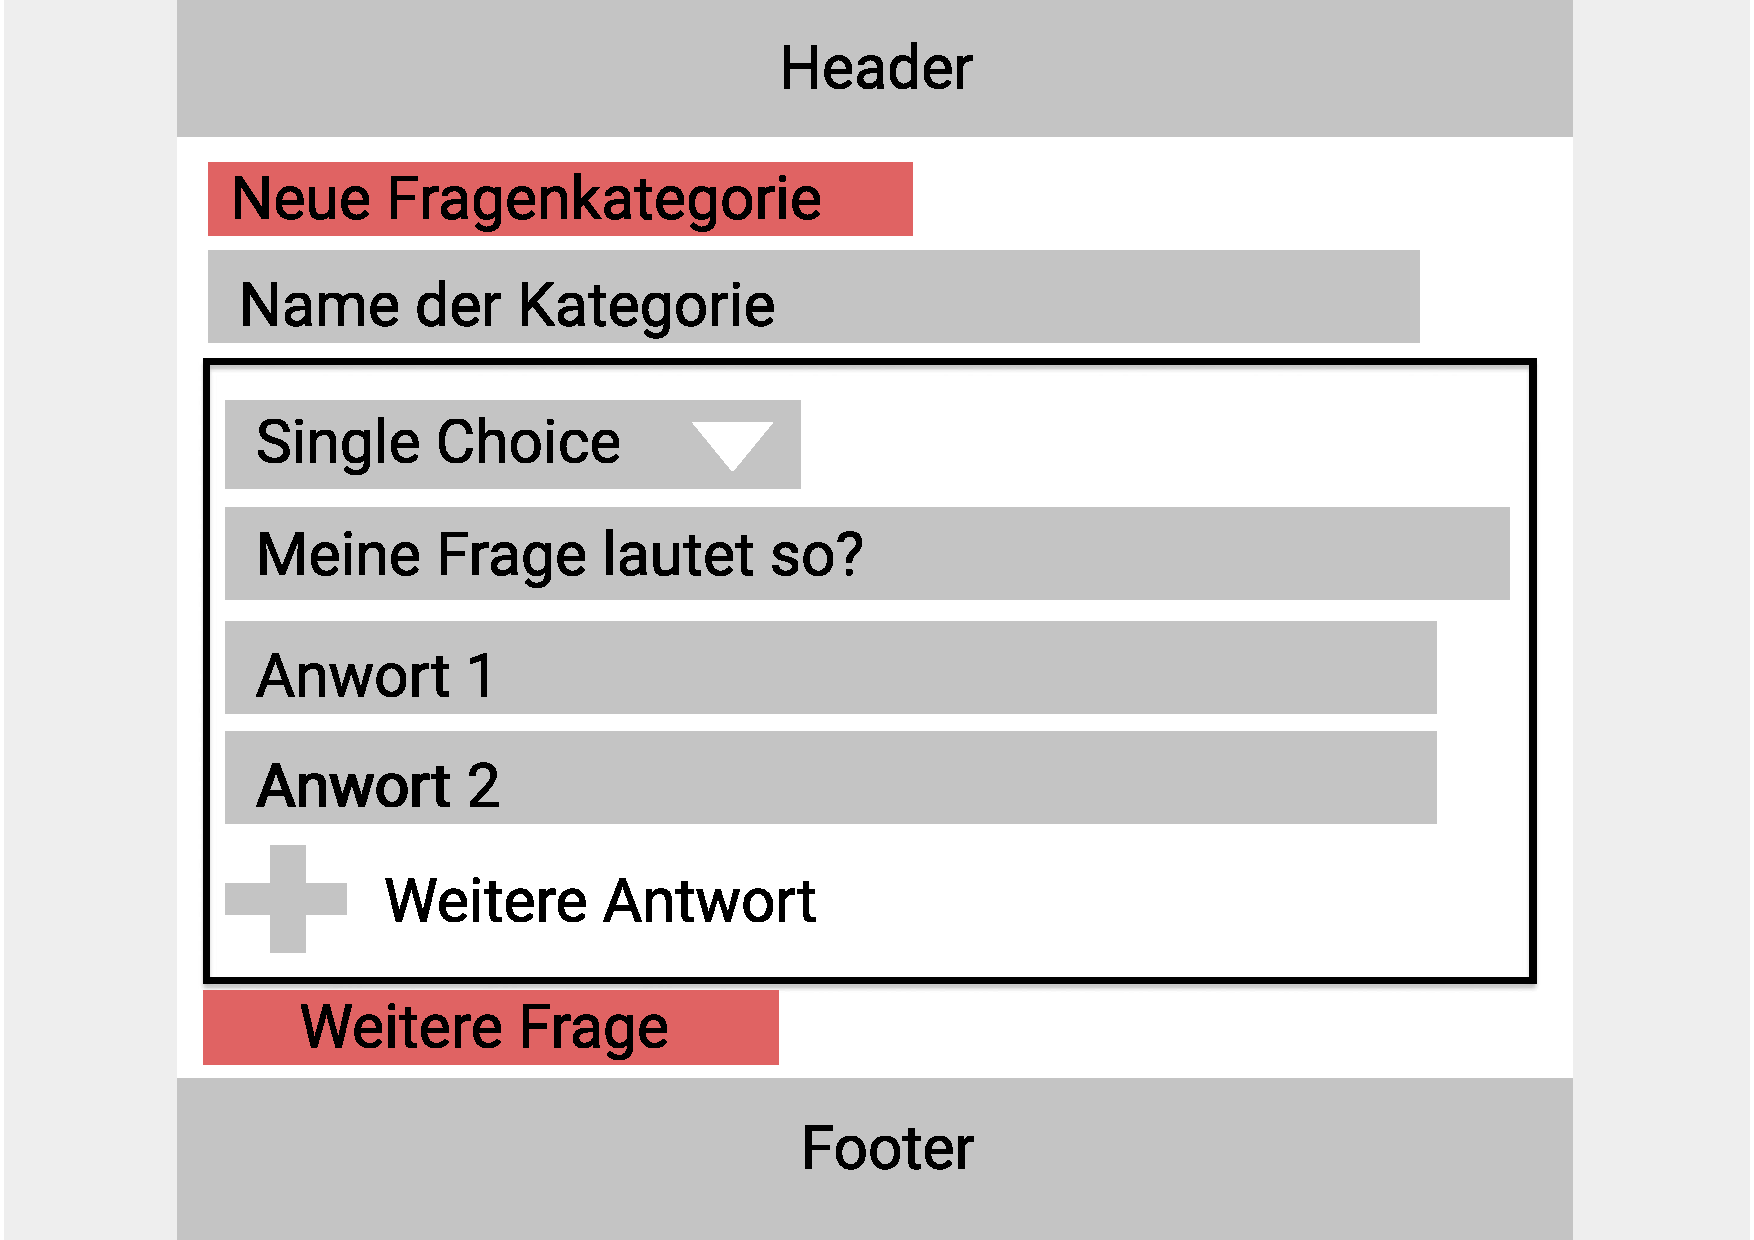
\includegraphics[width=0.7\textwidth]{img/konzeption/client/umfrage_erstellen_single_choice}
	\captionsetup{justification=centering, format=plain}
	\caption[Mock-Up der Umfrageerstellung von Single-Choice-Fragen]{Mock-Up der Umfrageerstellung von Single-Choice-Fragen\\\figma}
	\label{fig:MockUmfrageSingleChoice}
\end{figure}

\begin{figure}[H]
	\centering
	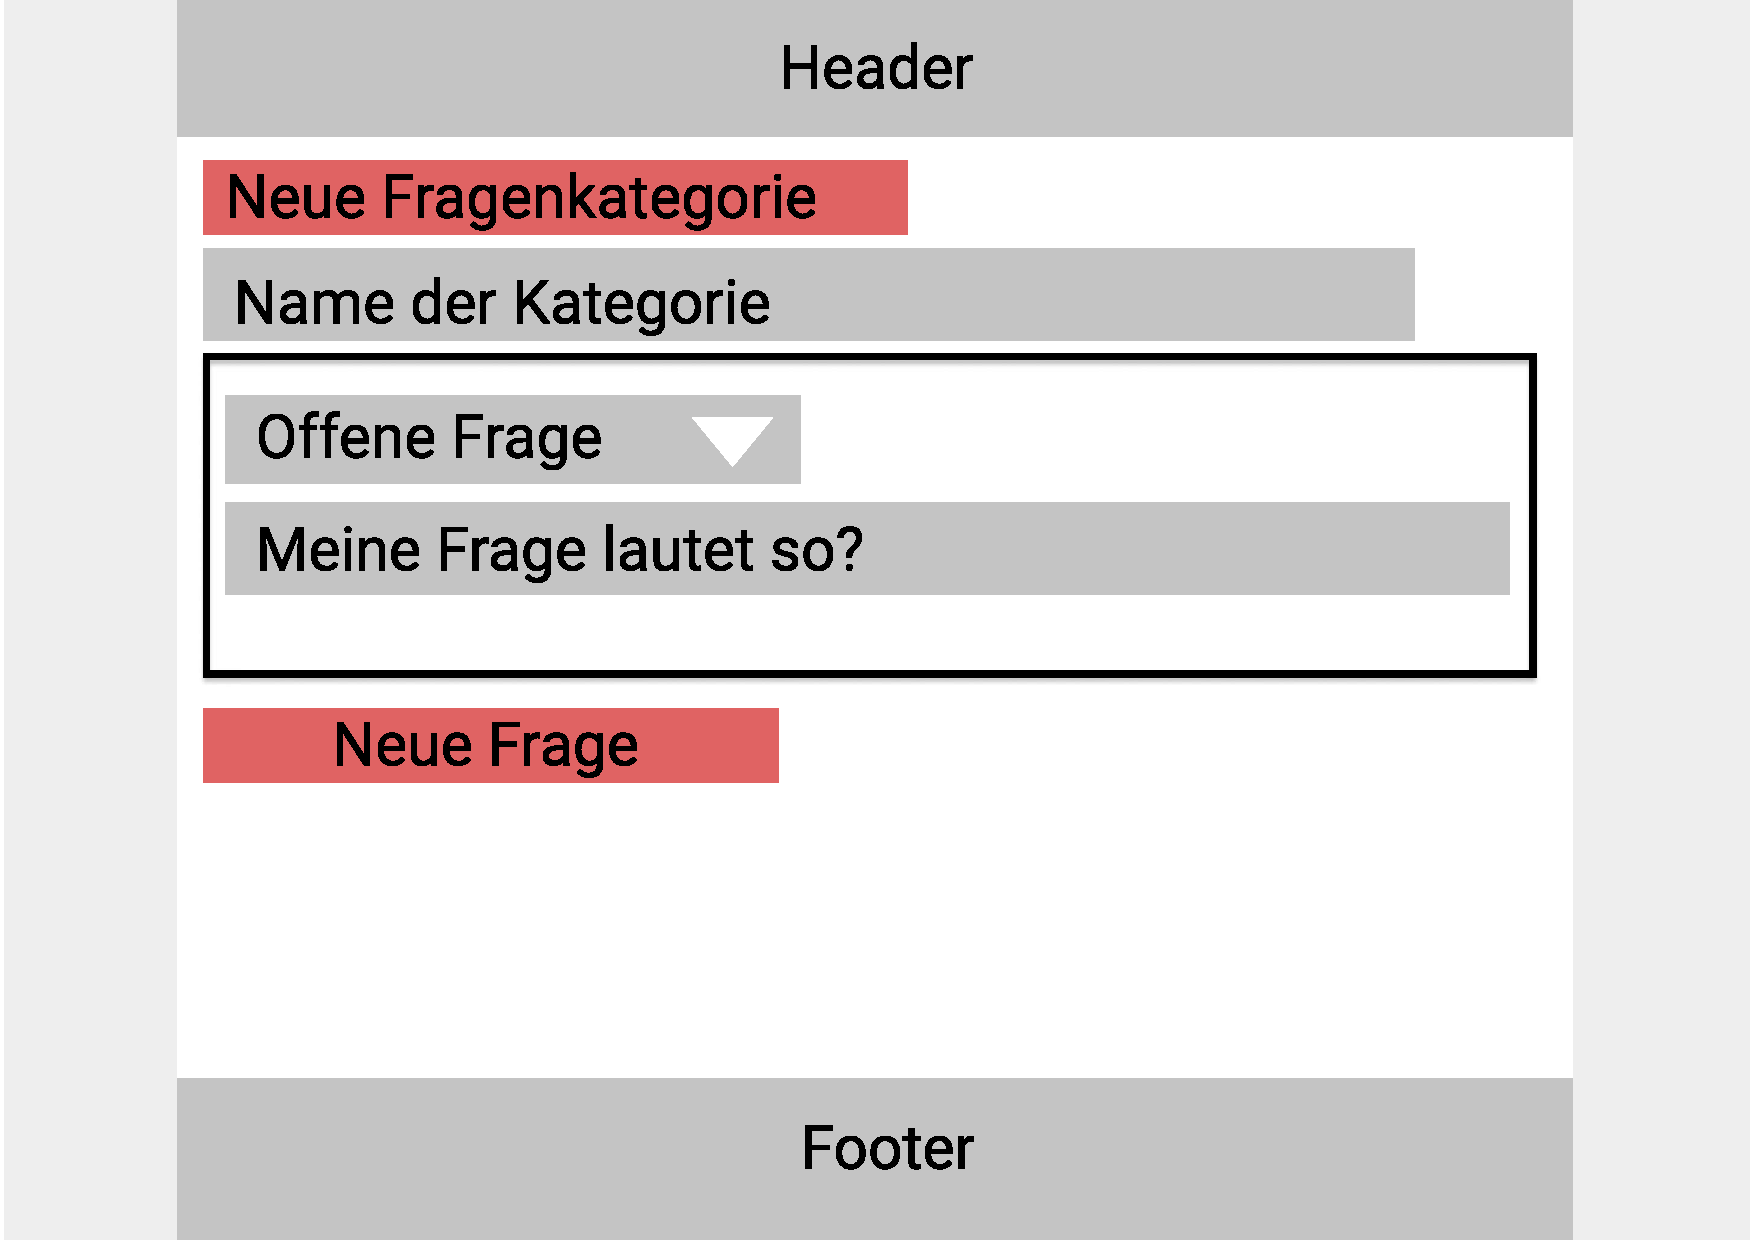
\includegraphics[width=0.7\textwidth]{img/konzeption/client/umfrage_erstellen_offene_frage}
	\captionsetup{justification=centering, format=plain}
	\caption[Mock-Up der Umfrageerstellung von offenen Fragen]{Mock-Up der Umfrageerstellung von offenen Fragen\\\figma}
	\label{fig:MockUmfrageOffeneFragen}
\end{figure}
